Let $P, Q$ be different points in $\mathbb{R}^3$, and let $\mathcal{P}$ be the collection of 3-vectors $\mathbf{v}$ with the same distance from $P$ and from $Q$: 
\[
\|\mathbf{P} - \mathbf{v}\| = \|\mathbf{Q} - \mathbf{v}\|.
\]

\begin{enumerate}
    \item[(a)] By squaring both sides of the distance equality and using that $\|\mathbf{w}\|^2 = \mathbf{w} \cdot \mathbf{w}$, show that $\mathcal{P}$ consists of exactly those 3-vectors $\mathbf{v}$ satisfying
    \[
    \mathbf{v} \cdot (\mathbf{P} - \mathbf{Q}) = \frac{1}{2} \left(\|\mathbf{P}\|^2 - \|\mathbf{Q}\|^2\right).
    \]

    In particular, the plane $\mathcal{P}$ has (nonzero) normal direction $\mathbf{P} - \mathbf{Q}$. Draw a picture to illustrate why it is reasonable that this is a plane with normal direction $\mathbf{P} - \mathbf{Q}$.

    Solution:

    \[\|\mathbf{P} - \mathbf{v}\| = \|\mathbf{Q} - \mathbf{v}\|.\]
    Squaring both sides:
    
 
      \[\|\mathbf{P}\|^2 +  \|\mathbf{v}\|^2 - 2(\mathbf{P}\cdot \mathbf{v})= \|\mathbf{Q}\|^2 +  \|\mathbf{v}\|^2 - 2(\mathbf{Q}\cdot \mathbf{v})\] 
        
        Rearranging the terms
        
       \[
    \mathbf{v} \cdot (\mathbf{P} - \mathbf{Q}) = \frac{1}{2} \left(\|\mathbf{P}\|^2 - \|\mathbf{Q}\|^2\right).
    \]
    
    See diagram below:

   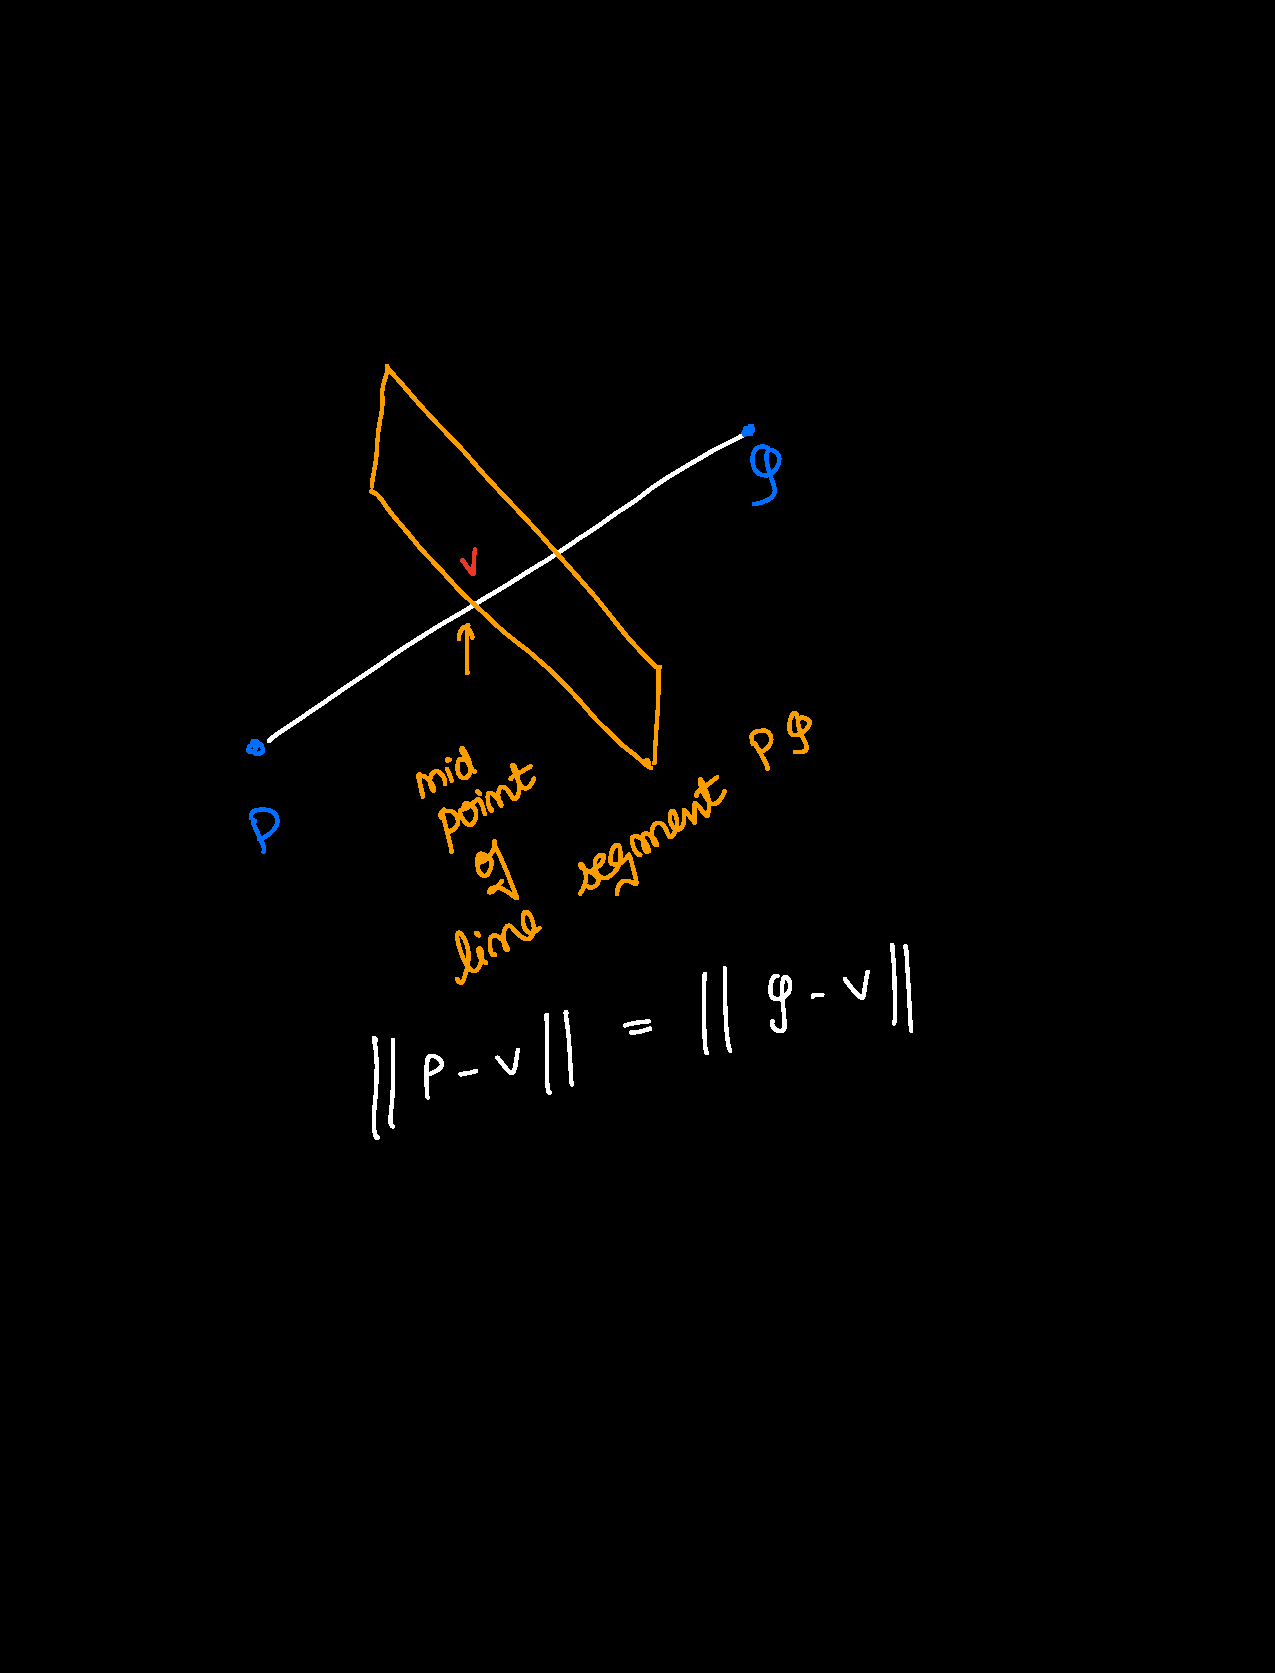
\includegraphics[width=\textwidth]{./diagrams/exercise_3_5_1.pdf}
    

    \item[(b)] For the case $\mathbf{P} = \begin{bmatrix} 3 \\ 4 \\ 3 \end{bmatrix}$ and $\mathbf{Q} = \begin{bmatrix} -1 \\ 5 \\ -2 \end{bmatrix}$, give an explicit equation for the plane $\mathcal{P}$.

   We have 
      \[
    \mathbf{v} \cdot (\mathbf{P} - \mathbf{Q}) = \frac{1}{2} \left(\|\mathbf{P}\|^2 - \|\mathbf{Q}\|^2\right).
    \]

    
\[
P =
\begin{bmatrix}
    3 \\ 4 \\ 3
\end{bmatrix}, Q = \begin{bmatrix}
    -1 \\ 5 \\ -2
\end{bmatrix}
\]
\[
P - Q = \begin{bmatrix}
    4 \\ -1 \\ 5
\end{bmatrix}
\]
\[
\|(\mathbf{P}\|)^2 = (3^2+4^2+3^2) = (9+16+9) = 34
\]
\[
\|(\mathbf{Q}\|)^2 = ((-1)^1+(5)^2+(-2)^2) = (1+25+4) = 30
\]
Let \[
 \mathbf{v} = \begin{bmatrix}
    x \\ y \\ z
\end{bmatrix}
\]
be any point on the plane.
\[
    \mathbf{v} \cdot (\mathbf{P} - \mathbf{Q}) = \frac{1}{2} \left(\|\mathbf{P}\|^2 - \|\mathbf{Q}\|^2\right).
\]
 \[
  \begin{bmatrix}
    x \\ y \\ z
\end{bmatrix} \cdot  \begin{bmatrix}
    4 \\ -1 \\ 5
\end{bmatrix} =  \frac{1}{2} \left(\|\mathbf{P}\|^2 - \|\mathbf{Q}\|^2\right)
\]
 \[
  \begin{bmatrix}
    x \\ y \\ z
\end{bmatrix} \cdot  \begin{bmatrix}
    4 \\ -1 \\ 5
\end{bmatrix} =  \frac{34-30}{2}  = 2
\]
Equation for the plane $\mathcal{P}:$
\[
4x - y + 5z = 2
\]
\end{enumerate}



